\chapter{REGULARIZATION METHODS FOR SUBSET ARMA SELECTION}

\section{INTRODUCTION}

Let $\{y_t: t=1,2,\cdots,T\}$ be a sequentially observed discrete and equally-spaced sample from a weakly stationary and homoskedastic process $\{Y_t:t=\cdots,-1,0,1,\cdots\}$. For the purpose of forecasting future realizations i.e. $\hat{y}_{t+h}$ where $h\in\mathbb{N}$, we estimate a model for $\{Y_t\}$ of the general form $Y_{t}=f(Y_{t-1},Y_{t-2},\cdots,Y_{t-p},\epsilon_{t-1},\epsilon_{t-2},\cdots,\epsilon_{t-q})+\epsilon_t$ from known $\{y_t\}$. Under homoskedasticitcy, $\{\epsilon_t\}$ is assumed to be white noise with mean 0 and variance $\sigma^2$.  Finite order parameters $p$ and $q$  quantify the extent of past information of $\{Y_t\}$ and $\{\epsilon_t\}$, respectively, helpful for prediction. Define $m=\max\{p,q\}$. In most cases, $m$ is small relative to $T$; however, when cyclical phenomenon is detected, $m=S$ where $S$ is the seasonal periodicity. The latter scenario often produces long gaps between relevant past information for model fit.

Common practice subset of the seasonal autoregressive moving average (SARMA) process is most commonly used for modeling the temporal dynamics of $\{y_t\}$ to forecast future unknown realizations. 

expressed in Equation \ref{eq:sarma} and abbreviated SARMA$(p,q)\times(P,Q)_{S}$ .


\begin{equation}
\label{eq:sarma}
\Phi(B^S)\phi(B)y_t=\Theta(B^S)\theta(B)\epsilon_t
\end{equation}

\begin{equation}
\label{eq:arma}
\bigg(1-\sum\limits_{i=1}^{p}\phi_{i}B^i\bigg)y_{t}=\bigg(1+\sum\limits_{j=1}^{q}\theta_{j}B^j\bigg)\epsilon_{t}
\end{equation}

In this parameterization, we utilize the backshift operator $B$ where $B^ky_{t}=y_{t-k}$. Furthermore, we assume $y_t$ has been centered and $\{\epsilon_t\}$ is white noise with zero mean and constant variance $\sigma^2$. Real-world application of the ARMA($p$,$q$) model to temporally dependent data relies on some form of model selection since model misspecification  

 Classically, the focus of model selection in this context identification of the AR order $p$ and MA order $q$.

For the purpose of subset ARMA selection, we express the model in Equation \ref{eq:arma} as the linear matrix form in Equation \ref{eq:linarma}. Under this $\bm{y}=\bm{X}\bm{\beta}+\bm{\epsilon}$
\begin{equation}
	\label{eq:linarma}
	\begin{bmatrix} y_m\\y_{m+1}\\y_{m+2}\\ \vdots\\ y_T\\ \end{bmatrix} =
	\begin{bmatrix} y_{m-1} & \cdots & y_{m-p} &
					\epsilon_{m-1} & \cdots & \epsilon_{m-q} \\
					y_{m-2} & \cdots & y_{m-p-1} &
					\epsilon_{m-2} & \cdots & \epsilon_{m-q-1} \\
					\vdots & \ddots & \vdots &
					\vdots & \ddots & \vdots & \\
					y_{T-1} & \cdots & y_{T-p} &
					\epsilon_{T-1} & \cdots & \epsilon_{T-q} \\
	\end{bmatrix}
	\begin{bmatrix} \phi_1\\ \phi_2\\ \vdots\\ \phi_p\\ \theta_1 \\
  						\theta_2\\ \vdots	\\ \theta_q\\ \end{bmatrix} +
  	\begin{bmatrix} \epsilon_m\\ \epsilon_{m+1}\\ \epsilon_{m+2}\\ \vdots\\ \epsilon_T\\ \end{bmatrix}
\end{equation}




\cite{Chen2011} 


\section{METHODS}

\subsection{ADAPTIVE LASSO}
The lease absolute shrinkage and selection operator (LASSO) of \cite{Tibshirani1996}.The $\L_1$ penalty is limited when highly correlated predictor variables are considered in model matrix $\bm{X}$.

Generally, the LASSO estimator $\hat{\bm{\beta}}$ is conditionally consistent for $\bm{\beta}$ 
\cite{Zhao2006}.
In \cite{Zou2006}

\subsection{ADAPTIVE ELASTIC NET}


\subsection{OPTIONS FOR SELECTING TUNING PARAMETERS}
Let $\mathcal{M}_1$ and $\mathcal{M}_2$ represent two competing subset ARMA($p$,$q$) models

Penalized estimation via E-NET of autoregressive parameters $\hat{\bm{\phi}}_{\lambda,\alpha}$ and $\hat{\bm{\theta}}_{\lambda,\alpha}$ using LASSO or ENET are dependent on selection of tuning parameters $\lambda$ and  $\alpha$.

\subsubsection{SELECTION BASED ON AIC OR BIC}

\subsubsection{SELECTION BASED ON OOS FORECAST EVALUATION}

\begin{figure}[htbp!]
	\caption{Variations of Out-of-Sample Procedures for Model Selection}
	\label{fig:oosplots}
	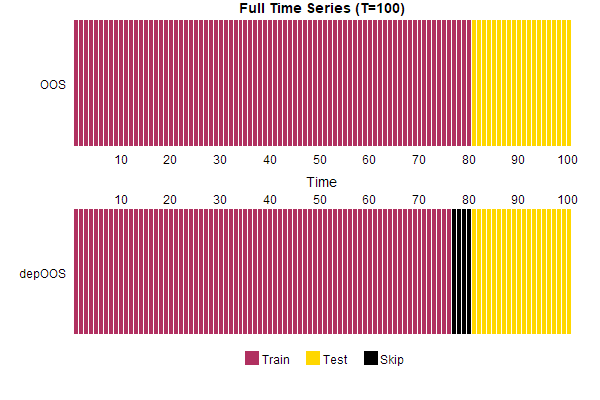
\includegraphics[scale=0.7]{oosplots}
\end{figure}

\subsubsection{SELECTION BASED ON CV FOR INDEPENDENT DATA}

\begin{figure}[htbp!]
	\caption{General $K$-fold Cross-Validation for Model Selection for $K=5$ (top) and $K=10$ (bottom)}
	\label{fig:kcvplots}
	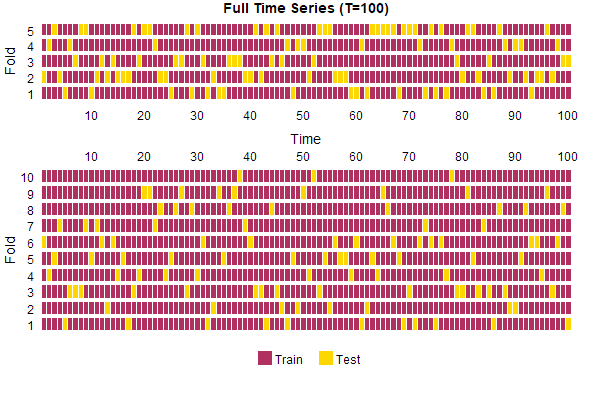
\includegraphics[scale=0.7]{kcvplots}
\end{figure}

\subsubsection{SELECTION BASED ON CV FOR DEPENDENT DATA}

\begin{figure}[htbp!]
	\caption{Non-Dependent $K$-fold Cross-Validation for Model Selection for $K=5$ (top) and $K=10$ (bottom)}
	\label{fig:depkcvplots}
	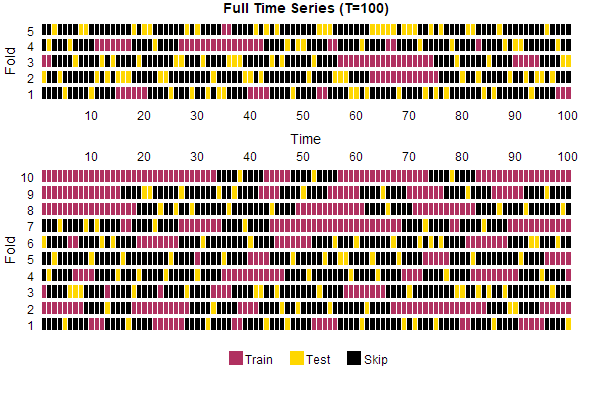
\includegraphics[scale=0.7]{depkcvplots}
\end{figure}

\begin{figure}[htbp!]
	\caption{Leave-One-Block-Out Cross-Validation for Model Selection}
	\label{fig:lobocvplots}
	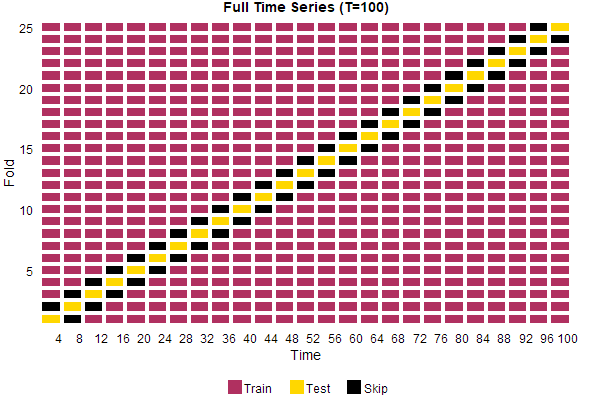
\includegraphics[scale=0.7]{lobocvplots}
\end{figure}

In the time series context, the best model minimizes forecasting error for future observations  unrealized during the model building  

\subsection{BAYESIAN PREDICTIVE POSTERIOR PROJECTION METHOD}
The classic method for model selection within the Bayesian framework begins with a reparameterization of the AR and MA coefficients to $\phi_i^*=\phi_i$ and $\theta_j^*=\theta_j$.

Since the introduction of Bayesian LASSO, research in Bayesian regularization methods has exploded over the last ten years. Bayesian methods analogous to adaptive lasso \citep{Leng2014}, elastic net \citep{Li2010a}, and adaptive elastic net \citep{Stankiewicz2015} have been introduced and applied. \cite{Polson2010}





\section{MONTE CARLO SIMULATIONS}
Multiple Monte Carlo studies are performed to evaluate the effectiveness of the three methods on subset ARMA selection. Consider the three time series $\{y_{1,t}\}$, $\{y_{2,t}\}$, and $\{y_{3,t}\}$ generated by the Gaussian ARMA processes expressed in Equations \ref{eq:simarma1}, \ref{eq:simarma2}, and \ref{eq:simarma3}.
\begin{equation}
	\label{eq:simarma1}
	y_{1,t}=0.8y_{1,t-1}+0.7y_{1,t-6}-0.56y_{1,t-7}+\epsilon_{1,t}
\end{equation}
\begin{equation}
	\begin{split}
	\label{eq:simarma2}
	y_{2,t}&=0.8y_{2,t-1}+0.7y_{2,t-6}-0.56y_{2,t-7}\\
	&+0.8\epsilon_{2,t-1}+0.7\epsilon_{2,t-6}+0.56\epsilon_{2,t-7}+\epsilon_{2,t}
	\end{split}
\end{equation}
\begin{equation}
	\label{eq:simarma3}
	y_{3,t}=0.8\epsilon_{3,t-1}+0.7\epsilon_{3,t-6}+0.56\epsilon_{3,t-7}+\epsilon_{3,t}
\end{equation}
The errors $\{\epsilon_{1,t}\}$, $\{\epsilon_{2,t}\}$, and $\{\epsilon_{3,t}\}$ are i.i.d. Gaussian processes with $0$ mean. These three ARMA models are equivalent to the multiplicative seasonal models of period 6 estimated in \cite{Chen2011} using adaptive Lasso. 





\section{APPLICATION}






\section{CONCLUSION}
